%
%  Kontkat-Daten
%==============================================================================
%==============================================================================
\chapter{Anhang}

%------------------------------------------------------------------------------
\section{Anhang Richtlinie}
%\newpage
%------------------------------------------------------------------------------
% - - - - - - - - - - - - - - - - - - - - - 
\begin{figure}[!h]
   \begin{center}
   \fbox{
      \includegraphics[width=0.85\textwidth,angle=0]% Achtung pdf muss schon Hochkant sein !
      {anhang/KontaktDaten.pdf}
      }
      \caption{\label{fig:KontaktDaten}
               Wichtige Namen, Anschriften und Telefonnummnern}
   \end{center}
 \end{figure}
 
\clearpage

%------------------------------------------------------------------------------
%\section{Zeit- und Arbeitsplan}
%\label{sec:BeispielPlan}
% - - - - - - - - - - - - - - - - - - - - - 
\begin{figure}[!h]
   \begin{center}
   \fbox{
      \includegraphics[width=0.85\textwidth,angle=0]% Achtung pdf muss schon Hochkant sein !
      {anhang/BspTerminplan.pdf}
      }
      \caption{\label{fig:BspPlan}
               Beispiel f�r Zeit- und Arbeitsplan}
   \end{center}
 \end{figure}
 
\clearpage
% - - - - - - - - - - - - - - - - - - - - - 
 \begin{figure}[!h]
   \begin{center}
   \fbox{
      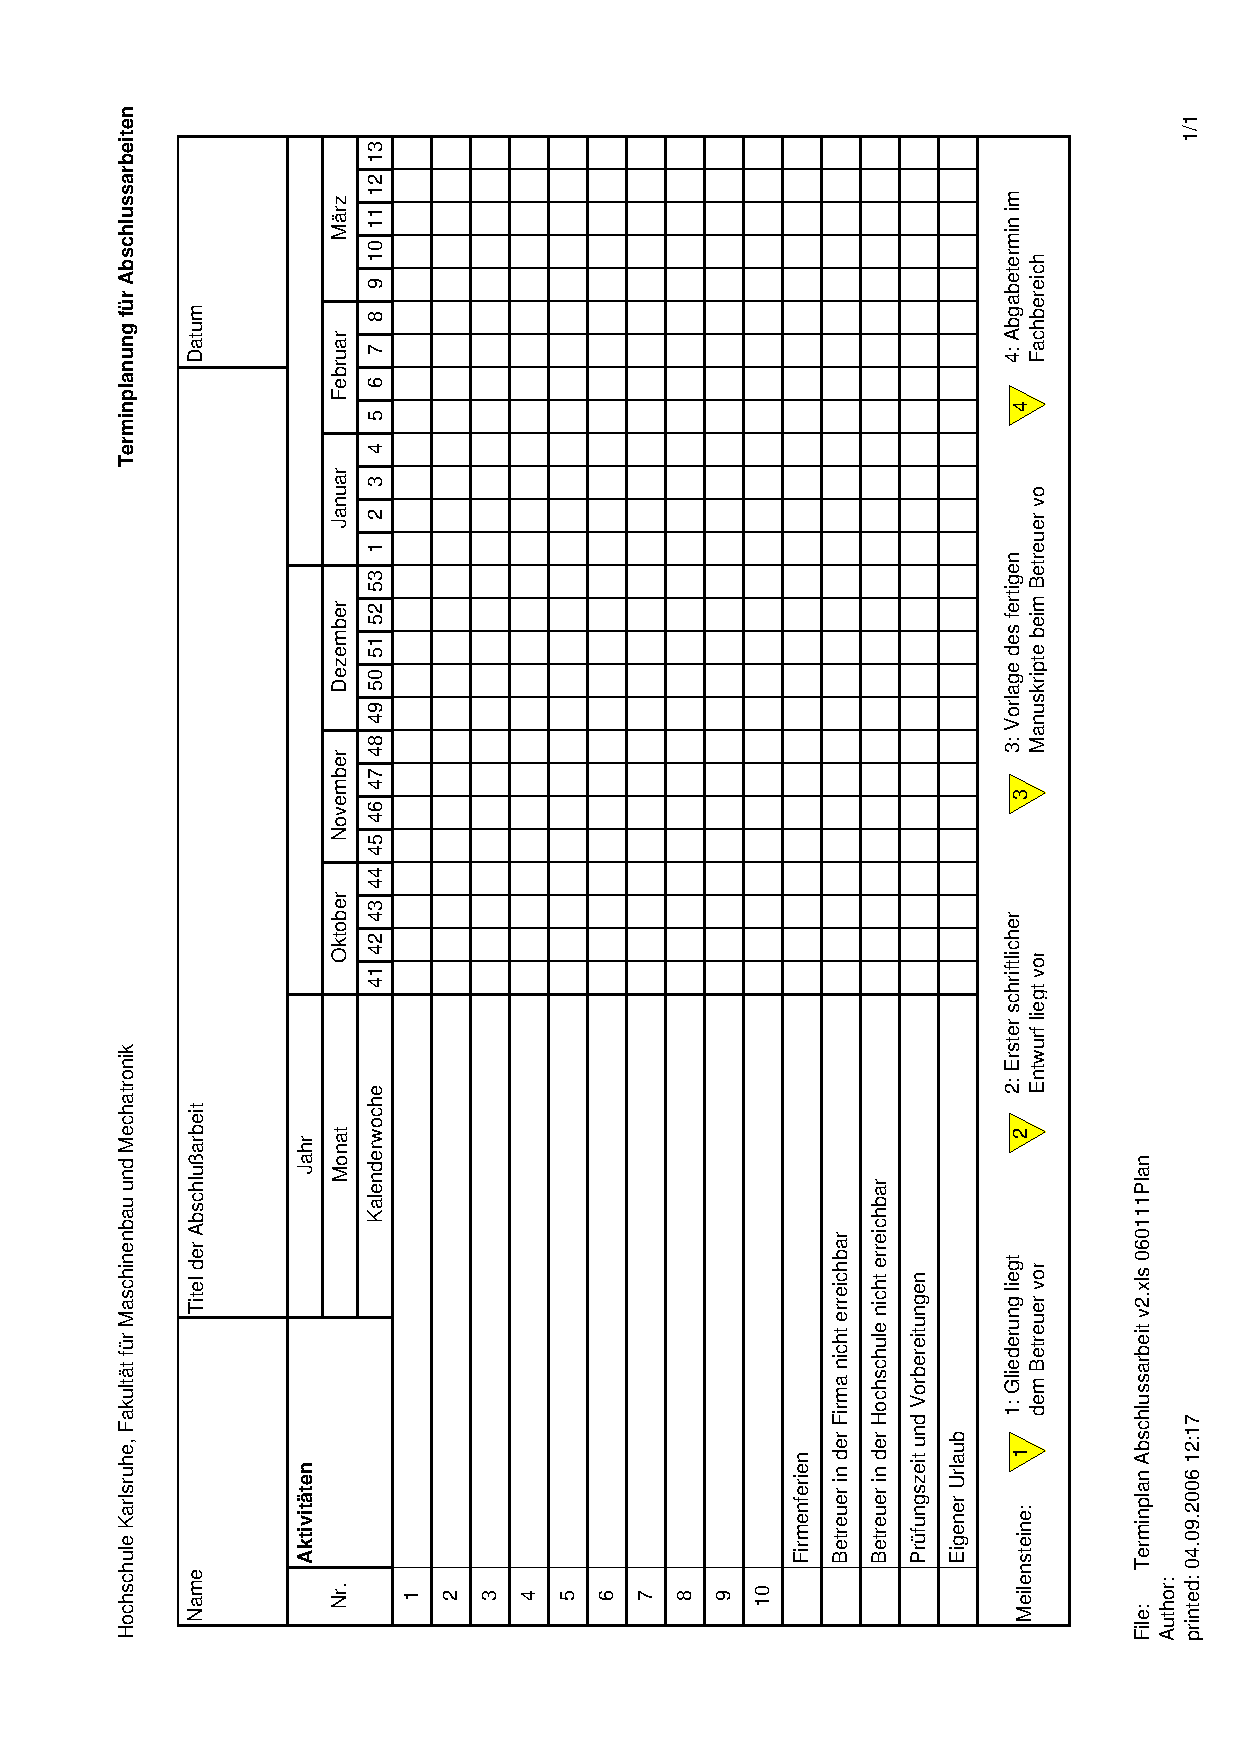
\includegraphics[width=0.85\textwidth,angle=0]
      {anhang/Terminplan_Abschlussarbeit_v2.pdf}
      }
      \caption{\label{fig:Plan}
               Vorlage f�r Zeit- und Arbeitsplan}
   \end{center}
 \end{figure}

\clearpage

%------------------------------------------------------------------------------
%\section{Titelseite}
%\label{sec:Titelseite}
% - - - - - - - - - - - - - - - - - - - - - 
 \begin{figure}[!h]
   \begin{center}
   \fbox{
      \includegraphics[width=0.85\textwidth, angle=0]{anhang/Titelseite}
      }
      \caption{\label{fig:Titelseite}
               Muster f�r die Titelseite}
   \end{center}
 \end{figure}

\clearpage

%------------------------------------------------------------------------------
%\section{Deckblatt}
%\label{sec:Deckblatt}

% - - - - - - - - - - - - - - - - - - - - - 
 \begin{figure}[!h]
   \begin{center}
   \fbox{
      \includegraphics[width=0.85\textwidth, angle=0]{anhang/Deckblatt}
        }     
      \caption{\label{fig:Deckblatt}
               Muster f�r das Deckblatt}
   \end{center}
 \end{figure}
 
 \clearpage
 
%------------------------------------------------------------------------------
%\section{Erkl�rung und Sperrvermerk}
%\label{sec:Erklaerung}
 
% - - - - - - - - - - - - - - - - - - - - -  
 \begin{figure}[!h]
   \begin{center}
   \fbox{
      \includegraphics[width=0.85\textwidth, angle=0]{anhang/Erkl�rung_Sperrvermerk}
        }     
      \caption{\label{fig:Erklaerung}
               Erkl�rung und Beispiel f�r Sperrvermerk}
   \end{center}
 \end{figure}
 
 \clearpage
 
%------------------------------------------------------------------------------
%\section{Inhaltsverzeichnis}
%\label{sec:Inhaltsverzeichnis}
 
% - - - - - - - - - - - - - - - - - - - - -  
 \begin{figure}[!h]
   \begin{center}
   \fbox{
      \includegraphics[width=0.85\textwidth, angle=0]{anhang/BspInhaltsverzeichnis}
        }     
      \caption{\label{fig:BspInhaltsverzeichnis}
               Beispiel f�r eine Inhaltsverzeichnis}
   \end{center}
 \end{figure}
 
 \clearpage
 
%------------------------------------------------------------------------------
%\section{Zusammenfassung}
%\label{sec:Zusammenfassung}
 
% - - - - - - - - - - - - - - - - - - - - -  
 \begin{figure}[!h]
   \begin{center}
   \fbox{
      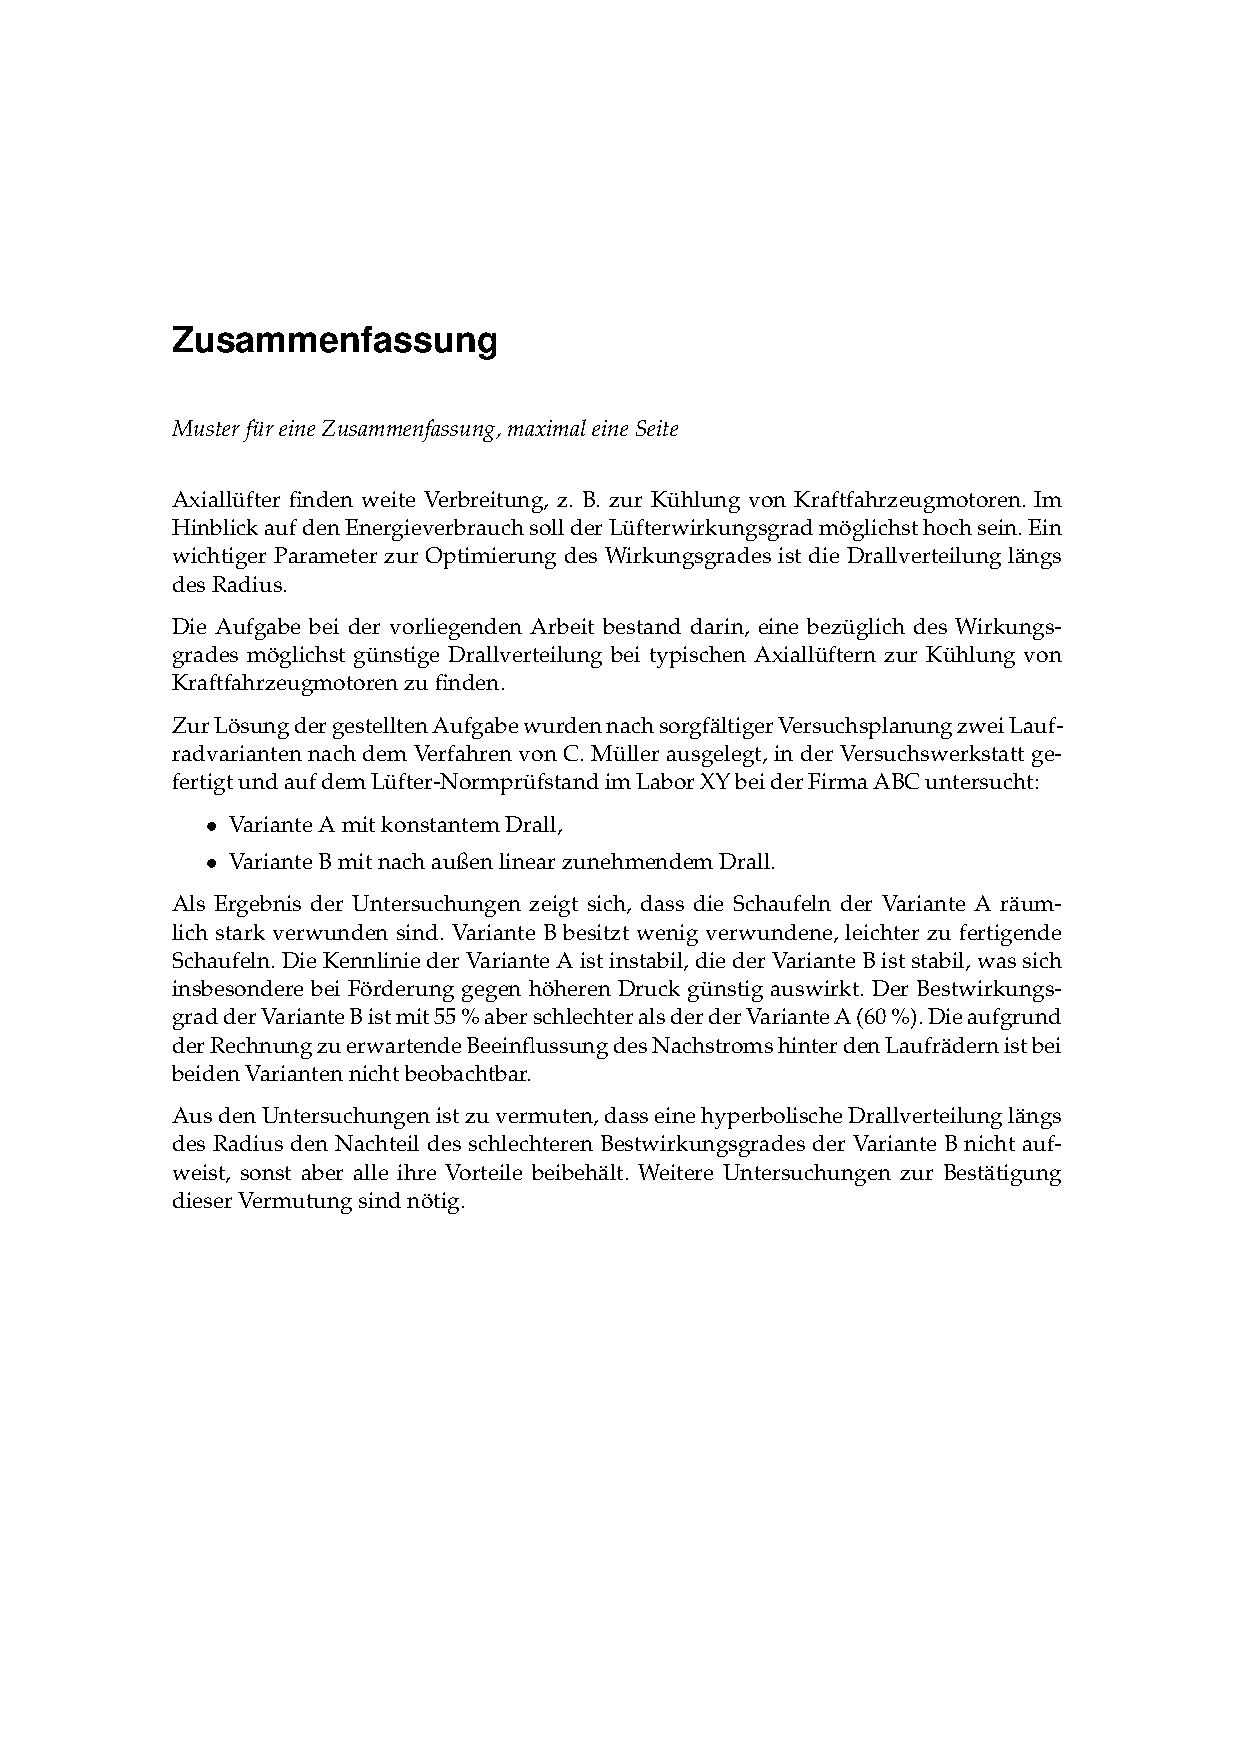
\includegraphics[width=0.85\textwidth, angle=0]{anhang/BspZusammenfassung}
        }     
      \caption{\label{fig:BspZusammenfassung}
               Beispiel f�r eine Zusammenfassung}
   \end{center}
 \end{figure}
 
 \clearpage
 
%------------------------------------------------------------------------------ 
%\section{Literaturverzeichnis}
%\label{sec:Literaturverzeichnis}
 
% - - - - - - - - - - - - - - - - - - - - -  
 \begin{figure}[!h]
   \begin{center}
   \fbox{
      \includegraphics[width=0.85\textwidth, angle=0]{anhang/BspLitVerzeichnis}
        }     
      \caption{\label{fig:BspLitVerzeichnis}
               Beispiel f�r ein Literaturverzeichnis}
   \end{center}
 \end{figure}
 
 \clearpage
%------------------------------------------------------------------------------   